\upaper{58}{Life Establishment on Urantia}
\author{Life Carrier}
\vs p058 0:1 In all Satania there are only 61 worlds similar to Urantia, life\hyp{}modification planets. The majority of inhabited worlds are peopled in accordance with established techniques; on such spheres the Life Carriers are afforded little leeway in their plans for life implantation. But about one world in ten is designated as a \bibemph{decimal planet} and assigned to the special registry of the Life Carriers; and on such planets we are permitted to undertake certain life experiments in an effort to modify or possibly improve the standard universe types of living beings.
\usection{1.\bibnobreakspace Physical\hyp{}Life Prerequisites}
\vs p058 1:1 \bibemph{600,000,000} years ago the commission of Life Carriers sent out from Jerusem arrived on Urantia and began the study of physical conditions preparatory to launching life on world number 606 of the Satania system. This was to be our 606\ts{th} experience with the initiation of the Nebadon life patterns in Satania and our 60\ts{th}\fnst{\textbf{606\ts{th} ... 60\ts{th}}, It is interesting to note that the planet number (606) added to the number of experiment (60) is 666, known also as \bibemph{The Number of the Beast}, see Revelation 13:18. Also, see the clarification of John's vision at \bibref[47:10.2]{p047 10:2} and the note at \bibref[15:14.8]{p015 14:8}.} opportunity to make changes and institute modifications in the basic and standard life designs of the local universe.
\vs p058 1:2 \pc It should be made clear that Life Carriers cannot initiate life until a sphere is ripe for the inauguration of the evolutionary cycle. Neither can we provide for a more rapid life development than can be supported and accommodated by the physical progress of the planet.
\vs p058 1:3 The Satania Life Carriers had projected a sodium chloride pattern of life; therefore no steps could be taken toward planting it until the ocean waters had become sufficiently briny. The Urantia type of protoplasm can function only in a suitable salt solution. All ancestral life --- vegetable and animal --- evolved in a salt\hyp{}solution habitat. And even the more highly organized land animals could not continue to live did not this same essential salt solution circulate throughout their bodies in the blood stream which freely bathes, literally submerses, every tiny living cell in this “briny deep.”
\vs p058 1:4 Your primitive ancestors freely circulated about in the salty ocean; today, this same oceanlike salty solution freely circulates about in your bodies, bathing each individual cell with a chemical liquid in all essentials comparable to the salt water which stimulated the first protoplasmic reactions of the first living cells to function on the planet.
\vs p058 1:5 But as this era opens, Urantia is in every way evolving toward a state favourable for the support of the initial forms of marine life. Slowly but surely physical developments on earth and in adjacent space regions are preparing the stage for the later attempts to establish such life forms as we had decided would be best adapted to the unfolding physical environment --- both terrestrial and spatial.
\vs p058 1:6 Subsequently the Satania commission of Life Carriers returned to Jerusem, preferring to await the further breakup of the continental land mass, which would afford still more inland seas and sheltered bays, before actually beginning life implantation.
\vs p058 1:7 \pc On a planet where life has a marine origin the ideal conditions for life implantation are provided by a large number of inland seas, by an extensive shore line of shallow waters and sheltered bays; and just such a distribution of the earth’s waters was rapidly developing. These ancient inland seas were seldom over 150--180\,m deep, and sunlight can penetrate ocean water for more than 180\,m\fnst{\textbf{sunlight can penetrate ocean water for more than 180\,m}, The density of most liquids decreases with increasing temperature, but water is an exception to this rule. In the region of temperatures 0--3\,°C for the salty ocean water or 0--4\,°C for the fresh water, the density \bibemph{increases} with increasing temperature, reaching the maximum density at the temperature 3\,°C for the salty and 4\,°C for the fresh water respectively. Therefore, the warm water at the surface (say, having the temperature 2\,°C) is more dense than the cold water (say, at 1\,°C) underneath and moves down replacing it, thus ensuring that the temperature does not fall below 2--3\,°C all the way to the bottom. This is also the reason why a pond begins to freeze from the surface to the bottom and not the other way around, which would have been catastrophic for the survival of fish and other forms of life in the pond.}.
\vs p058 1:8 And it was from such seashores of the mild and equable climes of a later age that primitive plant life found its way onto the land. There the high degree of carbon in the atmosphere afforded the new land varieties of life opportunity for speedy and luxuriant growth. Though this atmosphere was then ideal for plant growth, it contained such a high degree of carbon dioxide that no animal, much less man, could have lived on the face of the earth.
\usection{2.\bibnobreakspace The Urantia Atmosphere}
\vs p058 2:1 The planetary atmosphere filters through to the earth about $5 \times 10^{-10}$ of the sun’s total light emanation. If the light falling upon North America were paid for at the rate of 2¢/kWh, the annual light bill would be upward of 800 quadrillion\fnst{\textbf{quadrillion} $=$ one thousand trillion, $10^{15}$.} dollars. Chicago’s bill for sunshine would amount to considerably over \$100,000,000 a day. And it should be remembered that you receive from the sun other forms of energy --- light is not the only solar contribution reaching your atmosphere. Vast solar energies pour in upon Urantia embracing wave lengths ranging both above and below the recognition range of human vision.
\vs p058 2:2 \pc The earth’s atmosphere is all but opaque to much of the solar radiation at the extreme ultraviolet end of the spectrum. Most of these short wave lengths are absorbed by a layer of ozone which exists throughout a level about 16\,km above the surface of the earth, and which extends spaceward for another 16\,km. The ozone permeating this region, at conditions prevailing on the earth’s surface, would make a layer only 2.5\,mm thick\fnst{\textbf{2.5\,mm thick}, The present (2000) estimate of the ozone layer thickness over the US is about 3\,mm.}; nevertheless, this relatively small and apparently insignificant amount of ozone protects Urantia inhabitants from the excess of these dangerous and destructive ultraviolet radiations present in sunlight. But were this ozone layer just a trifle thicker, you would be deprived of the highly important and health\hyp{}giving ultraviolet rays which now reach the earth’s surface, and which are ancestral to one of the most essential of your vitamins.
\vs p058 2:3 And yet some of the less imaginative of your mortal mechanists insist on viewing material creation and human evolution as an accident. The Urantia midwayers have assembled over 50,000 facts of physics and chemistry which they deem to be incompatible with the laws of accidental chance, and which they contend unmistakably demonstrate the presence of intelligent purpose in the material creation. And all of this takes no account of their catalogue of more than 100,000 findings outside the domain of physics and chemistry which they maintain prove the presence of mind in the planning, creation, and maintenance of the material cosmos.
\vs p058 2:4 Your sun pours forth a veritable flood of death\hyp{}dealing rays, and your pleasant life on Urantia is due to the “fortuitous” influence of more than two\hyp{}score apparently accidental protective operations similar to the action of this unique ozone layer.
\vs p058 2:5 Were it not for the “blanketing” effect of the atmosphere at night, heat would be lost by radiation so rapidly that life would be impossible of maintenance except by artificial provision.
\vs p058 2:6 \pc The lower 8 or 10\,km of the earth’s atmosphere is the troposphere; this is the region of winds and air currents which provide weather phenomena. Above this region is the inner ionosphere and next above is the stratosphere. Ascending from the surface of the earth, the temperature steadily falls for 9 or 12\,km, at which height it registers around -57\,°C. This temperature range of from -54\,°C to -57\,°C is unchanged in the further ascent for 64 km; this realm of constant temperature is the stratosphere. At a height of 72 or 80\,km, the temperature begins to rise, and this increase continues until, at the level of the auroral displays, a temperature of 649\,°C is attained, and it is this intense heat that ionizes the oxygen. But temperature in such a rarefied atmosphere is hardly comparable with heat reckoning at the surface of the earth. Bear in mind that 50\% of all your atmosphere is to be found in the first 5\,km. The height of the earth’s atmosphere is indicated by the highest auroral streamers --- about 643\,km.
\vs p058 2:7 Auroral phenomena are directly related to sunspots, those solar cyclones which whirl in opposite directions above and below the solar equator, even as do the terrestrial tropical hurricanes. Such atmospheric disturbances whirl in opposite directions\fnst{\textbf{opposite directions}, This is due to the direction of the Coriolis force $\vec{F}_{cor} = 2m\vec{v}\times\vec{\omega}$, see the figure.} when occurring above or below the equator.\tunemarkup{pictures}{\begin{figure}[H]\centering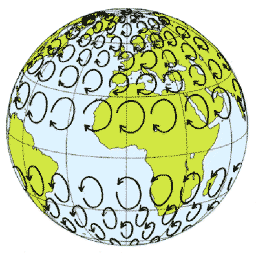
\includegraphics[width=0.5\columnwidth]{images/Coriolis-Effect.png}\caption{Coriolis effect}\end{figure}}
\vs p058 2:8 The power of sunspots to alter light frequencies shows that these solar storm centres function as enormous magnets. Such magnetic fields are able to hurl charged particles from the sunspot craters out through space to the earth’s outer atmosphere, where their ionizing influence produces such spectacular auroral displays. Therefore do you have the greatest auroral phenomena when sunspots are at their height --- or soon thereafter --- at which time the spots are more generally equatorially situated.
\vs p058 2:9 Even the compass needle is responsive to this solar influence since it turns slightly to the east as the sun rises and slightly to the west as the sun nears setting. This happens every day, but during the height of sunspot cycles this variation of the compass is twice as great. These diurnal wanderings of the compass are in response to the increased ionization of the upper atmosphere, which is produced by the sunlight.
\vs p058 2:10 It is the presence of two different levels of electrified conducting regions in the superstratosphere that accounts for the long\hyp{}distance transmission of your long\hyp{} and short\hyp{}wave radiobroadcasts. Your broadcasting is sometimes disturbed by the terrific storms which occasionally rage in the realms of these outer ionospheres.
\usection{3.\bibnobreakspace Spatial Environment}
\vs p058 3:1 During the earlier times of universe materialization the space regions are interspersed with vast hydrogen clouds, just such astronomic dust clusters as now characterize many regions throughout remote space. Much of the organized matter which the blazing suns break down and disperse as radiant energy was originally built up in these early appearing hydrogen clouds of space. Under certain unusual conditions atom disruption also occurs at the nucleus of the larger hydrogen masses. And all of these phenomena of atom building and atom dissolution, as in the highly heated nebulae, are attended by the emergence of flood tides of short space rays of radiant energy. Accompanying these diverse radiations is a form of space\hyp{}energy unknown on Urantia.
\vs p058 3:2 This short\hyp{}ray energy charge of universe space is 400 times greater than all other forms of radiant energy existing in the organized space domains. The output of short space rays, whether coming from the blazing nebulae, tense electric fields, outer space, or the vast hydrogen dust clouds, is modified qualitatively and quantitatively by fluctuations of, and sudden tension changes in, temperature, gravity, and electronic pressures.
\vs p058 3:3 These eventualities in the origin of the space rays are determined by many cosmic occurrences as well as by the orbits of circulating matter, which vary from modified circles to extreme ellipses. Physical conditions may also be greatly altered because the electron spin is sometimes in the opposite direction from that of the grosser matter behaviour, even in the same physical zone.
\vs p058 3:4 The vast hydrogen clouds are veritable cosmic chemical laboratories, harbouring all phases of evolving energy and metamorphosing matter. Great energy actions also occur in the marginal gases of the great binary stars which so frequently overlap and hence extensively commingle. But none of these tremendous and far\hyp{}flung energy activities of space exerts the least influence upon the phenomena of organized life --- the germ plasm of living things and beings. These energy conditions of space are germane to the essential environment of life establishment, but they are not effective in the subsequent modification of the inheritance factors of the germ plasm as are some of the longer rays of radiant energy. The implanted life of the Life Carriers is fully resistant to all of this amazing flood of the short space rays of universe energy.
\vs p058 3:5 \pc All of these essential cosmic conditions had to evolve to a favourable status before the Life Carriers could actually begin the establishment of life on Urantia.
\usection{4.\bibnobreakspace The Life\hyp{}Dawn Era}
\vs p058 4:1 That we are called Life Carriers should not confuse you. We can and do carry life to the planets, but we brought no life to Urantia. Urantia life is unique, original with the planet. This sphere is a life\hyp{}modification world; all life appearing hereon was formulated by us right here on the planet; and there is no other world in all Satania, even in all Nebadon, that has a life existence just like that of Urantia.
\vs p058 4:2 \pc \bibemph{550,000,000} years ago\fnst{\textbf{\bibemph{550,000,000} years ago}, This corresponds to the time when, according to Kislicyn's hypothesis, the geosphere underwent a deformation from the shape of a dodecahedron (the ``ether shape'') into the shape of an icosahedron (the ``water shape'').} the Life Carrier corps returned to Urantia. In co\hyp{}operation with spiritual powers and superphysical forces we organized and initiated the original life patterns of this world and planted them in the hospitable waters of the realm. All planetary life (aside from extraplanetary personalities) down to the days of Caligastia, the Planetary Prince, had its origin in our three original, identical, and simultaneous marine\hyp{}life implantations. These three life implantations have been designated as: the \bibemph{central} or Eurasian\hyp{}African, the \bibemph{eastern} or Australasian, and the \bibemph{western,} embracing Greenland and the Americas.
\vs p058 4:3 \pc \bibemph{500,000,000} years ago primitive marine vegetable life was well established on Urantia. Greenland and the arctic land mass, together with North and South America, were beginning their long and slow westward drift. Africa moved slightly south, creating an east and west trough, the Mediterranean basin, between itself and the mother body. Antarctica, Australia, and the land indicated by the islands of the Pacific broke away on the south and east and have drifted far away since that day.
\vs p058 4:4 We had planted the primitive form of marine life in the sheltered tropic bays of the central seas of the east\hyp{}west cleavage of the breaking\hyp{}up continental land mass. Our purpose in making three marine\hyp{}life implantations was to ensure that each great land mass would carry this life with it, in its warm\hyp{}water seas, as the land subsequently separated. We foresaw that in the later era of the emergence of land life large oceans of water would separate these drifting continental land masses.
\usection{5.\bibnobreakspace The Continental Drift}
\vs p058 5:1 The continental land drift continued. The earth’s core had become as dense and rigid as steel, being subjected to a pressure of almost $3.9 \times 10^{6}$ kg/cm\ts{2}, and owing to the enormous gravity pressure, it was and still is very hot in the deep interior. The temperature increases from the surface downward until at the centre it is slightly above the surface temperature of the sun.
\vs p058 5:2 The outer 1,600\,km of the earth’s mass consists principally of different kinds of rock. Underneath are the denser and heavier metallic elements. Throughout the early and preatmospheric ages the world was so nearly fluid in its molten and highly heated state that the heavier metals sank deep into the interior. Those found near the surface today represent the exudate of ancient volcanoes, later and extensive lava flows, and the more recent meteoric deposits.
\vs p058 5:3 The outer crust was about 64\,km thick. This outer shell was supported by, and rested directly upon, a molten sea of basalt of varying thickness, a mobile layer of molten lava held under high pressure but always tending to flow hither and yon in equalization of shifting planetary pressures, thereby tending to stabilize the earth’s crust.
\vs p058 5:4 Even today the continents continue to float upon this noncrystallized cushiony sea of molten basalt. Were it not for this protective condition, the more severe earthquakes would literally shake the world to pieces. Earthquakes are caused by sliding and shifting of the solid outer crust and not by volcanoes.
\vs p058 5:5 \pc The lava layers of the earth’s crust, when cooled, form granite. The average density of Urantia is a little more than 5.5 times that of water; the density of granite is less than 3 times that of water. The earth’s core is 12 times as dense as water.
\vs p058 5:6 The sea bottoms are more dense than the land masses, and this is what keeps the continents above water. When the sea bottoms are extruded above the sea level, they are found to consist largely of basalt, a form of lava considerably heavier than the granite of the land masses. Again, if the continents were not lighter than the ocean beds, gravity would draw the edges of the oceans up onto the land, but such phenomena are not observable.
\vs p058 5:7 The weight of the oceans is also a factor in the increase of pressure on the sea beds. The lower but comparatively heavier ocean beds, plus the weight of the overlying water, approximate the weight of the higher but much lighter continents. But all continents tend to creep into the oceans. The continental pressure at ocean\hyp{}bottom levels is about 1,400 kg/cm\ts{2}. That is, this would be the pressure of a continental mass standing 4,572\,m above the ocean floor. The ocean\hyp{}floor water pressure is only about 350 kg/cm\ts{2}. These differential pressures tend to cause the continents to slide toward the ocean beds.
\vs p058 5:8 Depression of the ocean bottom during the prelife ages had upthrust a solitary continental land mass to such a height that its lateral pressure tended to cause the eastern, western, and southern fringes to slide downhill, over the underlying semiviscous lava beds, into the waters of the surrounding Pacific Ocean. This so fully compensated the continental pressure that a wide break did not occur on the eastern shore of this ancient Asiatic continent, but ever since has that eastern coast line hovered over the precipice of its adjoining oceanic depths, threatening to slide into a watery grave.
\usection{6.\bibnobreakspace The Transition Period}
\vs p058 6:1 \bibemph{450,000,000} years ago the \bibemph{transition from vegetable to animal life} occurred. This metamorphosis took place in the shallow waters of the sheltered tropic bays and lagoons of the extensive shore lines of the separating continents. And this development, all of which was inherent in the original life patterns, came about gradually. There were many transitional stages between the early primitive vegetable forms of life and the later well\hyp{}defined animal organisms. Even today the transition slime moulds persist, and they can hardly be classified either as plants or as animals.
\vs p058 6:2 \pc Although the evolution of vegetable life can be traced into animal life, and though there have been found graduated series of plants and animals which progressively lead up from the most simple to the most complex and advanced organisms, you will not be able to find such connecting links between the great divisions of the animal kingdom nor between the highest of the prehuman animal types and the dawn men of the human races. These so\hyp{}called “missing links” will forever remain missing, for the simple reason that they never existed.
\vs p058 6:3 From era to era radically new species of animal life arise. They do not evolve as the result of the gradual accumulation of small variations; they appear as full\hyp{}fledged and new orders of life, and they appear \bibemph{suddenly.}
\vs p058 6:4 The \bibemph{sudden} appearance of new species and diversified orders of living organisms is wholly biologic, strictly natural. There is nothing supernatural connected with these genetic mutations.
\vs p058 6:5 At the proper degree of saltiness in the oceans animal life evolved, and it was comparatively simple to allow the briny waters to circulate through the animal bodies of marine life. But when the oceans were contracted and the percentage of salt was greatly increased, these same animals evolved the ability to reduce the saltiness of their body fluids just as those organisms which learned to live in fresh water acquired the ability to maintain the proper degree of sodium chloride in their body fluids by ingenious techniques of salt conservation.
\vs p058 6:6 Study of the rock\hyp{}embraced fossils of marine life reveals the early adjustment struggles of these primitive organisms. Plants and animals never cease to make these adjustment experiments. Ever the environment is changing, and always are living organisms striving to accommodate themselves to these never\hyp{}ending fluctuations.
\vs p058 6:7 The physiologic equipment and the anatomic structure of all new orders of life are in response to the action of physical law, but the subsequent endowment of mind is a bestowal of the adjutant mind\hyp{}spirits in accordance with innate brain capacity. Mind, while not a physical evolution, is wholly dependent on the brain capacity afforded by purely physical and evolutionary developments.
\vs p058 6:8 Through almost endless cycles of gains and losses, adjustments and readjustments, all living organisms swing back and forth from age to age. Those that attain cosmic unity persist, while those that fall short of this goal cease to exist.
\usection{7.\bibnobreakspace The Geologic History Book}
\vs p058 7:1 The vast group of rock systems which constituted the outer crust of the world during the life\hyp{}dawn or Proterozoic era does not now appear at many points on the earth’s surface. And when it does emerge from below all the accumulations of subsequent ages, there will be found only the fossil remains of vegetable and early primitive animal life. Some of these older water\hyp{}deposited rocks are commingled with subsequent layers, and sometimes they yield fossil remains of some of the earlier forms of vegetable life, while on the topmost layers occasionally may be found some of the more primitive forms of the early marine\hyp{}animal organisms. In many places these oldest stratified rock layers, bearing the fossils of the early marine life, both animal and vegetable, may be found directly on top of the older undifferentiated stone.
\vs p058 7:2 Fossils of this era yield algae, corallike plants, primitive Protozoa, and spongelike transition organisms. But the absence of such fossils in the early rock layers does not necessarily prove that living things were not elsewhere in existence at the time of their deposition. Life was sparse throughout these early times and only slowly made its way over the face of the earth.
\vs p058 7:3 \pc The rocks of this olden age are now at the earth’s surface, or very near the surface, over about \bibfrac{1}{8}\ts{th} of the present land area. The average thickness of this transition stone, the oldest stratified rock layers, is about 2.4\,km. At some points these ancient rock systems are as much as 6.4\,km thick, but many of the layers which have been ascribed to this era belong to later periods.
\vs p058 7:4 In North America this ancient and primitive fossil\hyp{}bearing stone layer comes to the surface over the eastern, central, and northern regions of Canada. There is also an intermittent east\hyp{}west ridge of this rock which extends from Pennsylvania and the ancient Adirondack Mountains on west through Michigan, Wisconsin, and Minnesota. Other ridges run from Newfoundland to Alabama and from Alaska to Mexico.
\vs p058 7:5 The rocks of this era are exposed here and there all over the world, but none are so easy of interpretation as those about Lake Superior and in the Grand Canyon of the Colorado River, where these primitive fossil\hyp{}bearing rocks, existing in several layers, testify to the upheavals and surface fluctuations of those faraway times.
\vs p058 7:6 This stone layer, the oldest fossil\hyp{}bearing stratum in the crust of the earth, has been crumpled, folded, and grotesquely twisted as a result of the upheavals of earthquakes and the early volcanoes. The lava flows of this age brought much iron, copper, and lead up near the planetary surface.
\vs p058 7:7 There are few places on the earth where such activities are more graphically shown than in the St. Croix valley of Wisconsin. In this region there occurred 127 successive lava flows on land with succeeding water submergence and consequent rock deposition. Although much of the upper rock sedimentation and intermittent lava flow is absent today, and though the bottom of this system is buried deep in the earth, nevertheless, about 65--70 of these stratified records of past ages are now exposed to view.
\vs p058 7:8 \pc In these early ages when much land was near sea level, there occurred many successive submergences and emergences. The earth’s crust was just entering upon its later period of comparative stabilization. The undulations, rises and dips, of the earlier continental drift contributed to the frequency of the periodic submergence of the great land masses.
\vs p058 7:9 During these times of primitive marine life, extensive areas of the continental shores sank beneath the seas from 1 to 800\,m. Much of the older sandstone and conglomerates represents the sedimentary accumulations of these ancient shores. The sedimentary rocks belonging to this early stratification rest directly upon those layers which date back far beyond the origin of life, back to the early appearance of the world\hyp{}wide ocean.
\vs p058 7:10 Some of the upper layers of these transition rock deposits contain small amounts of shale or slate of dark colours, indicating the presence of organic carbon and testifying to the existence of the ancestors of those forms of plant life which overran the earth during the succeeding Carboniferous or coal age. Much of the copper in these rock layers results from water deposition. Some is found in the cracks of the older rocks and is the concentrate of the sluggish swamp water of some ancient sheltered shore line. The iron mines of North America and Europe are located in deposits and extrusions lying partly in the older unstratified rocks and partly in these later stratified rocks of the transition periods of life formation.
\vs p058 7:11 \pc This era witnesses the spread of life throughout the waters of the world; marine life has become well established on Urantia. The bottoms of the shallow and extensive inland seas are being gradually overrun by a profuse and luxuriant growth of vegetation, while the shore\hyp{}line waters are swarming with the simple forms of animal life.
\vs p058 7:12 \pc All of this story is graphically told within the fossil pages of the vast “stone book” of world record. And the pages of this gigantic biogeologic record unfailingly tell the truth if you but acquire skill in their interpretation. Many of these ancient sea beds are now elevated high upon land, and their deposits of age upon age tell the story of the life struggles of those early days. It is literally true, as your poet has said, “The dust we tread upon was once alive.”
\vsetoff
\vs p058 7:13 [Presented by a member of the Urantia Life Carrier Corps now resident on the planet.]
\quizlink
